\documentclass[11pt, letterpaper]{article}

% Includes
\usepackage{acronym}
\usepackage{amsmath, amssymb, longtable, dcolumn}
\usepackage{bm}
\usepackage{color,soul}
\usepackage{colortbl}
\usepackage{csvsimple}
\usepackage{enumitem}
\usepackage{fancyhdr}
\usepackage{fullpage}
\usepackage{hyperref}
\usepackage{IEEEtrantools} % Requires sudo apt-get install texlive-publishers texlive-publishers-doc
\usepackage{indentfirst}
\usepackage{graphicx}
%\usepackage{lgrind}
\usepackage{multirow}
\usepackage{nccmath}  % Provides \medmath to change math size
\usepackage{pdfpages}
\usepackage{siunitx}
%\usepackage{subcaption}
\usepackage[caption=false,font=footnotesize]{subfig}
%\usepackage{subfigure}
%\usepackage{stfloats}  % Written by Sigitas Tolusis
\usepackage{tabularx}
\usepackage{units}
\usepackage{url}

% Use only one of the next two
%\usepackage{cite}
\usepackage{natbib}

% Setup
\newcommand{\doctitle}{CUSV Modeling}
\addtolength{\headheight}{2em}
\addtolength{\headsep}{1.5em}
\lhead{\doc}
\rhead{}
\setcounter{secnumdepth}{4}
\graphicspath{{images/}}
\newcommand{\capt}[1]{\caption{\small \em #1}}
\cfoot{\small Brian Bingham \today \\ \thepage}
\renewcommand{\footrulewidth}{0.4pt}

\newenvironment{xitemize}{\begin{itemize}\addtolength{\itemsep}{-0.75em}}{\end{itemize}}
\newenvironment{tasklist}{\begin{enumerate}[label=\textbf{\thesubsubsection-\arabic*},ref=\thesubsubsection-\arabic*,leftmargin=*]}{\end{enumerate}}

\makeatletter
\newcommand*{\compress}{\@minipagetrue}

% For using overleaf or local compilation
% See setting of true/false directly after \begin{document}
\newif\ifoverleaf % default is \overleaftrue

\begin{document}

\overleaffalse

% set the figure default size
\newcommand{\SF}{0.2}
\newcommand{\SFb}{0.45}
\newcommand{\SFPic}{0.45}
\newcommand{\SFPlot}{0.45}
\newcommand{\SFc}{0.25}
% Just a lazy way of setting the figure width (percentage of text width)
% 0.7 works well for 1 column
% 0.4 works well for 2 column
\newcommand{\FigWidth}{\SFb}

\newpage
% Title Page
%\setcounter{page}{1}
\begin{center}
{\huge \doctitle}
\end{center}

\section{Vehicle Model}
%
To approximate the motion of a surface vehicle in the ocean environment, we adapt the six degree-of-freedom robot-like vectorial model for marine craft, proposed by \citet{fossen11handbook}, and expressed as\footnote{The rigid-body terms can be expressed equivalently using either the total vessel velocity or the velocity relative the fluid, see Property 8.1 of \citet{fossen11handbook}.  For our implementation the rigid-body terms and the hydrodynamics terms are solved for separately, and it is more direct to leverage the native physics engine in terms of total rigid-body velocity.}
\begin{equation}
\underbrace{\bm{M}_{RB}\dot{\bm{\nu}}+\bm{C}_{RB}(\bm{\nu})\bm{\nu}}_\text{rigid-body forces} + 
\underbrace{\bm{M}_A\dot{\bm{\nu}}_r + \bm{C}_A(\bm{\nu}_r)\bm{\nu}_r + 
  \bm{D}(\bm{\nu}_r)\bm{\nu}_r}_\text{hydrodynamic forces} + 
\underbrace{\bm{g}(\bm{\eta})}_\text{hydrostatic forces} 
 = \bm{\tau}_{propulsion}+\bm{\tau}_{wind}+\bm{\tau}_{waves}
\label{e:fossenmodel}
\end{equation}
where
\begin{IEEEeqnarray}{rCl}\IEEEyesnumber\label{e:estate}
    \bm{\eta} & = & [x, y, z, \phi, \theta, \psi]^T \IEEEyessubnumber \\
    \bm{\nu}  & = & [u, v, w, p, q, r]^T \IEEEyessubnumber
\end{IEEEeqnarray}
are the position and velocity vectors respectively for surge, sway, heave, roll, pitch and yaw.  The total velocity, $\bm{\nu}$, is the sum of an irrotational water current velocity, $\bm{\nu}_c$, and the vessel velocity relative to the fluid, $\bm{\nu}_r$, i.e., $\bm{\nu}=\bm{\nu}_r+\bm{\nu}_c$.  The forces and moments due to propulsion (control), wind, and waves are represented as $\bm{\tau}_{propulsion}$, $\bm{\tau}_{wind}$ and $\bm{\tau}_{waves}$.

Traditionally, surface vessel models are separated into \emph{maneuvering} models (representing the surge, sway and yaw degrees-of-freedom) and \emph{seakeeping} models (representing the heave, pitch and roll degrees-of-freedom). For the purposes of supporting the development of autonomy, it is important that the unified simulation model include \emph{both} maneuvering and seakeeping degrees-of-freedom. The maneuvering aspects of the model influence the vessel steering and control portion of the autonomy solution. The inclusion of the seakeeping aspect of the model is critical for exercising the sensory perception portion of the autonomy solution.

\section{Rigid-Body Terms}

We assume that the principal axis of inertia can be consider to be coincident with the center-of-mass of the vessel.  The vessel is symmetric about the $x--z$ plane (left-right symmetry), which implies that $I_{xy}=I{yx}=0$.  We also simplify by considering the vessel to be symmetric about the $x--y$ plane (top-bottom symmetry) such that $I_{xz}=0$.  The result is a diagonal inertia matrix.
\begin{equation}
\bm{M}_{RB}= \left[ 
\begin{array}{ccccccc}
m & 0 & 0 & 0 & 0 & 0 \\
0 & m & 0 & 0 & 0 & 0 \\
0 & 0 & 0 & 0 & 0 & 0 \\
0 & 0 & 0 & I_{xx} & 0 & 0 \\
0 & 0 & 0 & 0 & I_{yy} & 0 \\
0 & 0 & 0 & 0 & 0 & I_{zz} 
\end{array} \right].
\end{equation}
and a Coriolis-centripetal matrix
\begin{equation}
\bm{C}_{RB}(\bm{\nu})= \left[ 
\begin{array}{ccccccc}
  0 & 0 & 0 & 0 & mw & -mv \\
  0 & 0 & 0 & -mw & 0 & mu \\
  0 & 0 & 0 & mv & -mu & 0 \\
  0 & mw  & -mv & 0 & I_{zz}r & -I_{yy}q \\
  -mw & 0 & mu & -I_{zz}r & 0 & I_{xx}p \\
  mv & -mu & 0 & I_{yy}q & -I_{xx}p  & 0
\end{array} \right].
\end{equation}

\subsection{Parameter Estimation}

\begin{itemize}
\item Mass is calculated based on an estimate of draft, the effective length and the cross-section of a circle segment.  The value is consistent specifications of similar vessels.
\item Moments of inertia are based on an effective cylindrical model
\end{itemize}

\begin{table}
\renewcommand{\arraystretch}{1.3}
\caption{Mass properties}
\label{t:example}
\centering
\begin{tabular}{crll}
  \hline \hline
  Parameter & Value & Units & Description \\
  \hline  \hline
  \multicolumn{4}{c}{Given Values} \\
  \hline
  $L$ & 12.2 & \unit[]{m} & Length \\
  $B$ & 3.34 & \unit[]{m} & Beam \\
  $\rho$ & 1,024 & $\unit[]{kg/m^3}$ & Density of seawater \\
  \hline \hline \multicolumn{4}{c}{Estimated Values} \\
  \hline
  $T$ & 1.2 & \unit[]{m} & Draft \\
  \hline \hline \multicolumn{4}{c}{Calculated Values} \\
  \hline
  $A_{wp}$ & 35 & $\unit[]{m^2}$ & Waterplane area \\
  $\nabla$ & 32 & $\unit[]{m^3}$ & Displaced volume \\
  $m$ & 33,000 & $\unit[]{kg}$ & Mass \\
  $I_{xx}$ & 20,700 & $\unit[]{kg\cdot m^s}$ & Moment of inertia, roll \\
  $I_{yy}=I_{zz}$ & 420,000 & $\unit[]{kg\cdot m^s}$ & Moment of inertia, pitch and yaw \\
  \hline
\end{tabular}
\end{table}

\section{Hydrodynamic Terms}\label{s:hydro}
%
The hydrodynamic forces in \eqref{e:fossenmodel} include the added mass terms due to the inertia of the surrounding fluid and hydrodynamic damping terms due to the vehicle interacting with the surrounding fluid. The terms are captured using coefficients, typically referred to as hydrodynamic derivatives, and expressed using SNAME (1950) notation \citep{fossen11handbook}.

The added mass matrix for our vehicle model is expressed as
\begin{equation}\hspace{-0.15in}
\medmath{
\bm{M}_{A}= -\left[ 
\begin{array}{cccccc}
X_{\dot{u}} & 0 & 0 & 0 & 0 & 0 \\
0 & Y_{\dot{v}} & 0 & 0 & 0 & Y_{\dot{r}} \\
0 & 0  &Z_{\dot{w}} & 0 & 0 & 0 \\
0 & 0 & 0 &K_{\dot{p}} & 0 & 0 \\
0 & 0 & 0 & 0 &M_{\dot{q}} & 0 \\
0 & N_{\dot{v}} & 0 & 0 & 0 & N_{\dot{r}} 
\end{array} \right]
}
\end{equation}
where, according to \citet{fossen11handbook} we can assume $N_{\dot{v}} = Y_{\dot{r}}$ for a slow moving surface ship.


The surge, sway, yaw components of our model match the maneuvering model used by \citet{sarda16station}. For the heave, roll, pitch components, we follow the six degree-of-freedom coupled motion maneuvering model presented by \citet{fossen11handbook} that only contains the diagonal terms for these components. As noted by \citet{fossen11handbook}, the off-diagonal elements of the added mass matrix, $\bm{M}_{A}$, will be small compared to the diagonal elements for most hullforms.


Once the added mass terms that make up $\bm{M}_{A}$ are chosen, the derivation by \citet{imlay61complete} provides the Coriolis-centripetal added mass terms that result. The Coriolis-centripetal added mass matrix is expressed using the same hydrodynamic derivatives from $\bm{M}_{A}$. The resultant matrix is
\begin{equation}
    \medmath{\bm{C}_{A}(\bm{\nu}_r)=
    \left[ 
    \begin{array}{cccccc}
        0 & 0 & 0 & 0 & -Z_{\dot{w}}w_r & Y_{\dot{v}}v_r+Y_{\dot{r}}r \\
        0 & 0 & 0 & Z_{\dot{w}}w_r & 0 & -X_{\dot{u}}u_r\\       
        0 & 0 & 0 & -Y_{\dot{v}}v_r & X_{\dot{u}}u_r & 0 \\
        0 & -Z_{\dot{w}}w_r & Y_{\dot{v}}v_r & 0 & -N_{\dot{r}}r_r & M_{\dot{q}}q_r \\
        -Z_{\dot{w}}w_r & 0 & -X_{\dot{u}}u_r & N_{\dot{r}}r_r & 0 & -K_{\dot{p}}p_r \\
        -Y_{\dot{v}}v_r - Y_{\dot{r}}r & X_{\dot{u}}u_r & 0 & -M_{\dot{q}}q_r & K_{\dot{p}}p_r & 0 
    \end{array}
    \right].}
\end{equation}

Since the terms of the maneuvering portion of our unified model are chosen to match those of \citet{sarda16station}, we simply used their theoretical expressions to estimate the values for $X_{\dot{u}}$, $Y_{\dot{v}}$, $N_{\dot{r}}$, and $Y_{\dot{r}}$. To estimate the added mass terms in the seakeeping portion of our model we used the previous work of \citet{greenhow88added} involving the study of added mass and damping of partially submerged horizontal cylinders in heave and sway. From their work we were able to directly estimate the heave added mass, $Z_{\dot{w}}$, by assuming that each pontoon could be represented by a circular cylinder. For the roll and pitch added mass, we assumed that half of this added mass acted at half the beam, for roll, and a quarter of the length, for pitch.

The hydrodynamic damping includes forces due to radiation-induced potential damping, skin friction, wave drift damping, vortex shedding and lifting forces \citep{fossen11handbook,krishnamurthy05modeling}.  These effects are aggregated in the hydrodynamic damping matrix 
\begin{equation}
\bm{D}(\bm{\nu}_r) = \bm{D}_l+\bm{D}_n(\bm{\nu}_r)
\end{equation}
expressed as a sum of linear and quadratic terms:
\begin{equation}
  \medmath{
\bm{D}_l= -\left[ 
\begin{array}{cccccc}
X_{u} & 0     & 0     & 0     & 0     & 0\\
0     & Y_{v} & 0     & 0     & 0     & Y_{r}\\
0     & 0     & Z_{w} & 0     & 0     & 0 \\
0     & 0     & 0     & K_{p} & 0     & 0 \\
0     & 0     & 0     & 0     & M_{q} & 0 \\
0     & N_{v} & 0     & 0     & 0     & N_{r}
\end{array} \right]
}
\label{e:D}
\end{equation}
and
\begin{equation}\label{e:D_n}
  {
    \bm{D}_n(\bm{\nu}_r) =
    -\left[ 
      \begin{array}{cccccc}% *** did an ad-hoc horizontal spacing fix here; perhaps there's a more elegant solution
          X_{u|u|}|u_r| & \hspace{-0.25in}0 & 0 & 0 & 0 & \hspace{-0.10in}0 \\
          0 & \hspace{-0.25in}Y_{v|v|}|v_r| & 0 & 0 & 0 & \hspace{-0.10in}0  \\
          0 & \hspace{-0.25in}0 & 0 & 0 & 0 & \hspace{-0.10in}0   \\
          0 & \hspace{-0.25in}0 & 0 & 0 & 0 & \hspace{-0.10in}0  \\
          0 & \hspace{-0.25in}0 & 0 & 0 & 0 & \hspace{-0.10in}0  \\
          0 & \hspace{-0.25in}0 & 0 & 0 & 0 & \hspace{-0.10in}N_{r|r|}|r| 
      \end{array} \right].
  }
\end{equation}

As discussed in \citet{fossen11handbook}, for a surface vehicle, the linear damping matrix captures predominately two effects, viscous skin-friction damping and potential damping. In the maneuvering degrees-of-freedom, the viscous component of the linear damping term becomes the dominant damping contribution for vehicles traveling at low speed. In the seakeeping degrees of freedom the radiation-induced potential damping component is important because these motion components by a surface vehicle produce significant radiated waves. The potential damping for these degrees-of-freedom is important regardless of the forward speed. Unlike the horizontal plane, the vertical plane motions have restoring forces or moments and consequently occur at their natural frequencies which affects the speed of these motions more than the vehicle forward speed.

Our linear damping matrix, $\bm{D}_l$, contains terms to capture both of these effects. The maneuvering degrees-of-freedom terms, $X_{u}$, $Y_{v}$, and $N_{r}$, capture the low-speed skin-friction damping the vehicle experiences and were included in the linear damping matrix used by \citet{sarda16station}. To estimate these terms we use the theoretical expressions presented by them. Their model also contained the off-diagonal terms, $Y_{r}$ and $N_{v}$. Since we are utilizing their model we also include those terms and use the expressions they provided to estimate them. The remaining maneuvering off-diagonal terms are assumed to be negligible. The seakeeping degrees-of-freedom terms, $Z_{w}$, $K_{p}$, and $M_{q}$, capture the radiation-induced potential damping the vehicle experiences. To estimate these terms we used the potential damping results from \citet{greenhow88added} for a heaving partially submerged horizontal cylinder. The roll and pitch damping values assumed that half this damping occurred at the same length scales as used for the added mass estimates. All the seakeeping off-diagonal terms should be negligible and are not included in our model.

\citet{fossen11handbook} also highlighted that for a surface vehicle the nonlinear damping matrix, with its cross-flow damping terms, becomes the dominant damping contribution at high speed for the maneuvering degrees-of-freedom. Since we want our vehicle model to represent the behavior of a wide range of surface vehicles and operating conditions, we have included these nonlinear damping terms in our unified model. However, since the vehicle  is predominately a low speed vehicle, when we apply our unified model specifically, we set the $Y_{v|v|}$ and $N_{r|r|}$ terms to zero. We also normally set $X_{u|u|}$ to zero.

This approximation of the hydrodynamic effects is implemented as a parameterized Gazebo plugin.  The user defines the characteristics of the vessel under test through a vessel-specific configuration file that includes the hydrodynamic derivatives.  During each time step of the simulation, the plugin is executed with access to the state of the vessel and environment.  The hydrodynamic force terms in \eqref{e:fossenmodel} are calculated based on this state information and the user-defined vessel characteristics.  The resulting force and moment values are then applied to the vessel through the Gazebo application programming interface (API) for inclusion in the next iteration of the physics engine.

% maybe this paragraph is no longer needed???
This simplified six degree-of-freedom model and the Gazebo plugin are generally applicable to surface vessels.  Applying this model to a specific vessel requires determining values for the hydrodynamic derivatives.  These values can be approximated from first principles (e.g., potential flow theory) or estimated through experimental testing (e.g., scale model testing).  \citet{sarda16station} estimate the hydrodynamic derivatives for a three degree-of-freedom model of thevessel by manually tuning the coefficients so that the model outputs agree with experimental measurements from at-sea maneuvering tests.  Each of the of linear drag terms in  \eqref{e:D} are estimated, but only the surge term in the quadratic drag matrix \eqref{e:D_n} is identified, implying that the remaining quadratic terms are neglected.

\subsection{Drag Estimate}

The resistance $R$ do to any particular drag component is expressed as a drag coefficient $C_D$ were
\[
R = \frac{1}{2}C_D \rho S U^2
\]
where $S$ is the at-rest hull wetted surface and $\rho$ is the water density. The total ship drag, $C_T$ is expressed as
\[
C_T = C_W + (1+k) C_F
\]
where $C_w$ is the wve drag, $C_F$ is the frictional drag and $k$ is a form factor representing the viscous pressure drag some fraction of the frictional resistance coefficient.


\begin{table}
\renewcommand{\arraystretch}{1.3}
\caption{Hull-Form/Fineness Coefficients}
\label{t:hullform}
\centering
\begin{tabular}{llrl}
  \hline \hline
  Parameter & Symbol & Value & Units \\
  \hline  \hline
  \multicolumn{4}{c}{Given Values} \\
  \hline
  Length of waterline & $L$ & 12.2 & \unit[]{m} \\
  Beam on waterline & $B$ & 3.34 & \unit[]{m} \\
  \hline \hline \multicolumn{4}{c}{Estimated Values} \\
  \hline
  Draft &  $T$ & 1.2 & \unit[]{m} \\
  \hline \hline \multicolumn{4}{c}{Calculated Values} \\
  \hline
  Waterplane area & $A_{wp}$ & 35 & $\unit[]{m^2}$  \\
  Maximum section area & $A_X$ & 3.01 & $\unit[]{m^2}$  \\
  Midship section area & $A_M$ & 3.01 & $\unit[]{m^2}$  \\
  Wetted surface Area & $S$ & 51 & $\unit[]{m^2}$  \\
  Displaced volume & $\nabla$ & 32 & $\unit[]{m^3}$ \\
  \hline \hline \multicolumn{4}{c}{Hull-Form Coefficients} \\
  \hline
  Prismatic & $C_P = \frac{\nabla}{A_X L} $ & 0.875 &\\
  Volumetric & $C_V = \frac{\nabla}{L^3} $ & 0.018 &\\
  Maximum Section & $C_X = \frac{A_X}{BT} $ & 0.75 &\\
  Midship Section & $C_M = \frac{A_M}{BT} $ & 0.75 &\\
  Block & $C_B = \frac{\nabla}{LBT} $ & 0.66 &\\
  Vertical Prismatic & $C_{PV} = \frac{\nabla}{A_{WP}T} $ & 0.75 &\\
  Waterplane  & $C_{WP} = \frac{A_{WP}}{LB} $ & 0.875 &\\
  & $B/T$   & 2.8 & \\
  & $S/V^{2/3}$ & 5.1 \\
  \hline 
\end{tabular}
\end{table}

\begin{figure}[hbt!]
\centering
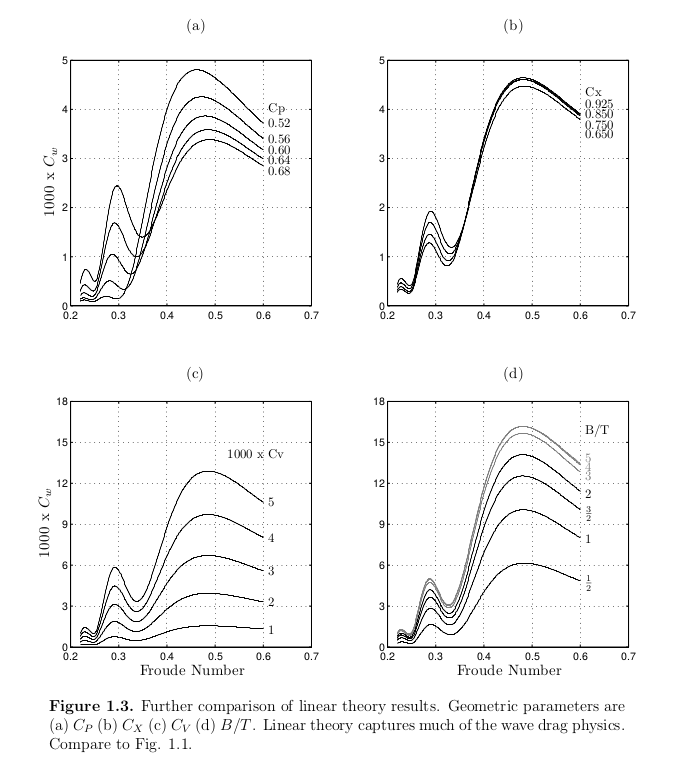
\includegraphics[width=0.6\linewidth]{drag_est.png}
\caption{\cite{read09drag}}
\label{f:drag_est}
\end{figure}


Holtrop's method suggests that the fritctional drag component can be neglected for normal  \cite{holtrop82approximate,holtrop84statistical}

\begin{itemize}
\item Assume a Froude number between $Fr=0.2--0.3$, which is $U=\unit[2.2--3.3]{m/s}$.
\item Figure~\ref{f:drag_est} suggests $C_w \approx \num{1.0e-3}$.
\item Using Holtrop's method \cite{holtrop82approximate,holtrop84statistical}, we calculate $(1+k) = 1.76$
  \item Using ITTC 1957 line/method $C_F = \frac{0.075}{(log_{10}(Re)-2)^2}$ suggest that  $C_w \approx \num{2.0e-3}$ which is consistent with the guideline that the majority of the hull's total resistance is due to water friction at slow speeds.
  \end{itemize}
The result is $C_T = \num{4.5e-3}$, the total resistance force is
\[
R = \frac{1}{2}C_T \rho S U^2  = 118.0 U^2
\]
So
\begin{itemize}
\item $X_u = 0$
\item $X_{u|u|}=\unit[118.0]{N/(m/s)^2}$
  \end{itemize}




\bibliographystyle{apalike}

\ifoverleaf
\bibliography{bbing_master}
\else
\bibliography{../latexlib/bib/bbing_master}
\fi

\end{document}

